\input sys/inputs.tex

\begin{document}

\bigheading{Kritikus munkák}

% \info{task_name}{infile}{outfile}{points}{timelimit}{memlimit}
% leave this values, if you are not interested
\info{critical}{stdin}{stdout}{100}{600 ms}{32 MiB}

Egy nagy építkezést $N$ elvégzendő munkára bontottak. Az építkezés vezetője függőségi feltételeket állapított meg a munkák között. Ez azt jelenti, hogy vannak olyan $u$ és $v$ munkapárok, hogy az $u$ munka befejezése meg kell hogy előzze a $v$ munka elkezdését. Ekkor azt mondjuk, hogy az $u$ munka \emph{közvetlenül megelőzi} a $v$ munkát. Azt mondjuk, hogy az $u$ munka \emph{megelőzi} a $v$ munkát, ha $u$ közvetlenül megelőzi $v$-t, vagy van olyan $z$ munka, hogy $u$ megelőzi $z$-t és $z$ megelőzi $v$-t.

Bármely $u$ munkát kritikusnak nevezünk, ha bármely ($u$-tól különböző) $v$ munka esetén vagy $v$ megelőzi $u$-t, vagy $u$ megelőzi $v$-t. Feltételezhető, hogy az építkezés elvégezhető a függőségi feltételek betartásával, azaz nincs olyan $u$ munka, amely megelőzné önmagát.

\heading{Feladat}

Írj programot, amely kiszámítja az összes kritikus munkát!

\heading{Bemenet}

A bemenet első sora két egész számot tartalmaz, $N$-et és $M$-et. $N$ a munkák száma ($1 \leq N \leq 100000$), $M$ pedig a függőségi feltételek száma ($0 \leq M \leq 1000000$). A munkákat az $1, \ldots ,N$ számok azonosítják. A következő $M$ sor mindegyike két egész számot tartalmaz, egy $u$ és $v$ közvetlen függőségi párt ($1 \leq u \neq v \leq N$), tehát $u$ közvetlenül megelőzi $v$-t.

\heading{Korlátok}

A tesztesetek $40 \%$-ában $N \leq 5000$ és $M \leq 30000$.


\heading{Kimenet}

A kimenet első sora a kritikus munkák számát tartalmazza. A második sor a kritikus munkák azonosítóit tartalmazza növekvő sorrendben egy-egy szóközzel elválasztva. Ha nincsen kritikus munka, akkor az első és egyetlen sor a 0 számot tartalmazza.


\heading{Példa bemenet és kimenet}

\sampleIN
7 9
1 3
2 3
3 4
3 5
4 6
5 6
1 7
3 7
7 4
\sampleOUT
2
3 6
\sampleCOMMENT

\sampleEND

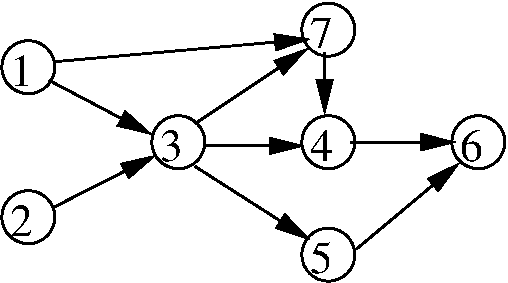
\includegraphics[height=4cm]{img/critical-fig.pdf}

\end{document}
